\chapter{Теоретическая часть и проектирование}
\section{Выбор движка}
Было принято решение использовать в качестве платформы игровой движок \emph{Unity}. Unity широко используется в компьютерных, консольных и мобильных играх, а также в приложениях дополненной и виртуальной реальности. Этот движок используется как крупными компаниями, так и независимыми разработчиками.

Главное преимущество игрового движка перед специализированным программным обеспечением для трёхмерного моделирования - это возможность генерировать деревья непосредственно в игре. Такой подход позволяет делать каждое дерево уникальным, что немаловажно при процедурной генерации уровней. Кроме того, отпадает необходимость экспорта и загрузки десятков разных моделей; для создания дерева достаточно прикрепить нужный компонент к игровому объекту. 

\section{Выбор стиля}
В качестве графического стиля был выбран \emph{low poly} - стиль, в котором намеренно используется низкое число полигонов для достижения угловатого и минималистичного внешнего вида. Как было сказано во введении, подобные модели строятся из геометрических примитивов и зачастую не используют текстуры, благодаря чему их гораздо проще создавать по сравнению с высокополигональными моделями. По тем же причинам они хорошо подходят для процедурной генерации. 

На рисунке ~\ref{fig:lowpoly} изображены модели деревьев, выполненные в этом стиле.

\begin{figure}[h]
    \centering
    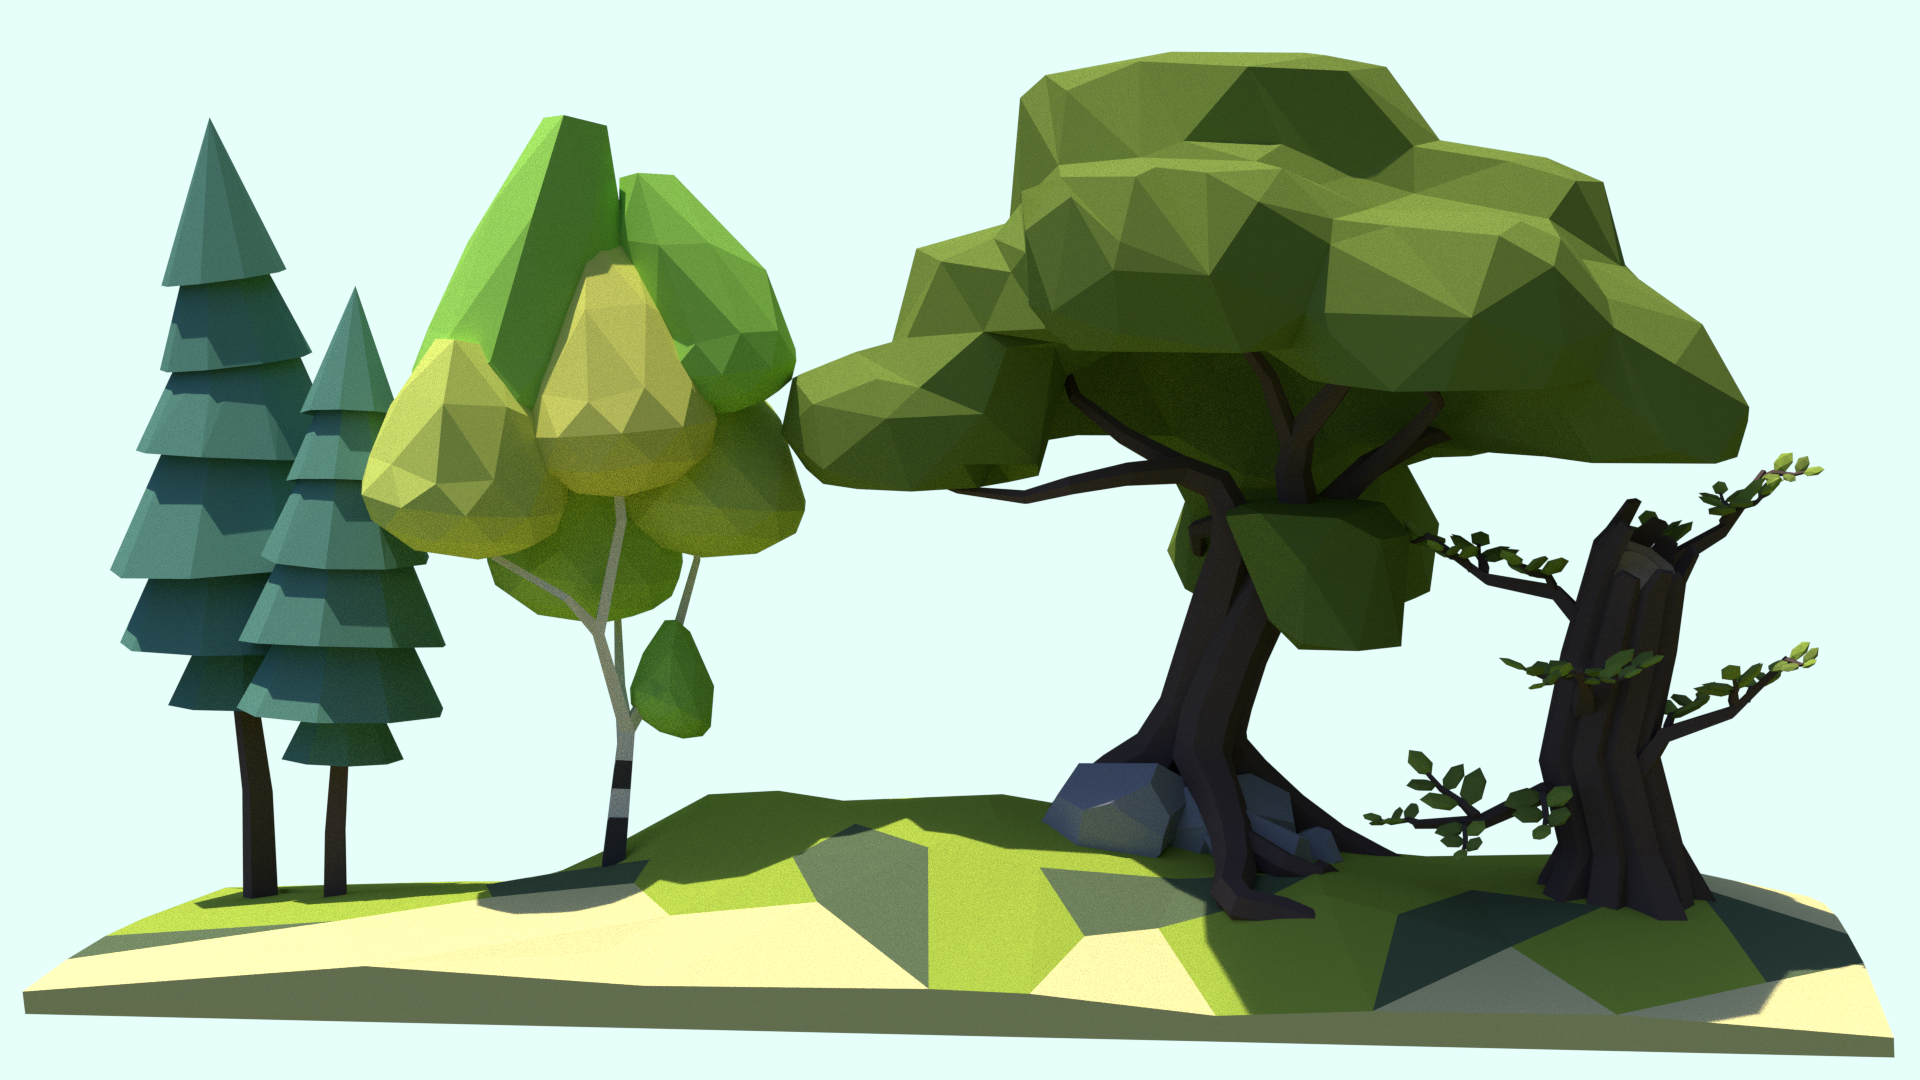
\includegraphics[width=0.8\textwidth]{lowpoly}
    \caption{Деревья в стиле Low poly. Автор: Lars Mezaka}
    \label{fig:lowpoly}
\end{figure}

Важной составляющей low poly является уровень детализации. Он должен поддерживаться на постоянном уровне. К примеру, если имеется модель камня и необходима модель камня меньшего размера, то использовать уменьшенную модель большого камня нежелательно, поскольку в этом случае маленький камень получится более детализированным и не будет сочетаться с остальной сценой визуально. Вместо этого лучше создать для него отдельную модель. Исходя из этого принципа, уровень детализации сгенерированных моделей будет выбираться автоматически в зависимости от параметров. К примеру, в стволе тонкого дерева будет меньше граней, чем в стволе более толстого.

\section{Описание движка Unity}
Unity - кроссплатформенный игровой движок, впервые выпущенный в 2005 году американской компанией Unity Technologies. В Unity применяется модульная система компонентов, позволяющая добавлять объектам необходимый функционал с помощью Drag-and-drop интерфейса. Для написания скриптов используется язык программирования C\#, работающий на свободной и кроссплатформенной реализации платформы .NET - Mono.

Ключевые особенности Unity - это наличие визуального редактора с множеством полезных инструментов для разработки и отладки приложений, возможность быстрого создания прототипов и поддержка более 25 платформ. Unity имеет несколько лицензий, одна из которых бесплатна и может использоваться при условии, что ежегодный доход от продажи игры не превышает 100000 долларов США. Редактор доступен для Windows и MacOS; с 2019 года доступна экспериментальная версия для Linux в независимом от дистрибутива формате AppImage.

\section{Структура 3D-модели}
Термины ``3D model'' (трёхмерная модель) и ``mesh'' (полигональная сетка) часто путают и используют как синонимы. Разница в том, что полигональная сетка содержит только информацию о геометрии, а модель, помимо полигональной сетки, может содержать и другую информацию, к примеру, анимацию или текстуры.

\emph{Полигональная сетка} - это совокупность вершин, рёбер и граней, которая определяет форму объекта. Помимо этого, полигональная сетка может содержать данные о нормалях, касательных, цветах вершин и \emph{UV-координатах}, которые применяются для наложения текстуры на сетку.

\emph{Грани} в трёхмерной графике являются многоугольниками. Чаще всего они имеют форму треугольника, потому что треугольник гарантированно лежит в одной плоскости, и благодаря этому свойству их проще обрабатывать и отрисовывать. 

Грани описываются \emph{массивом индексов вершин}, из которых они состоят. Зачем описывать вершины и грани по отдельности, если грань можно описать координатами вершин? Преимущество такого подхода в уменьшении использования памяти. Поскольку у смежных граней всегда будут общие вершины, дублирование данных в массиве неизбежно; однако при использовании индексов необходимо дублировать лишь 32 бита против 96 битов трёхмерного вектора, задающего вершину.

\section{Средства работы с полигональными сетками в Unity}
Трёхмерная модель в Unity представлена классом \texttt{Mesh}\cite{UnityMesh}. Его основные наборы данных - это массив вершин и массив треугольников.

Массив треугольников содержит тройки индексов вершин, образующих треугольник. Важной особенностью является то, что треугольник отрисовывается только в том случае, если порядок обхода вершин в проекции треугольника на экран соответствует обходу по часовой стрелке. Это правило удовлетворяет конвенции OpenGL и оптимизирует рендеринг, позволяя отсекать лишние грани, направленные против камеры.

Также \texttt{Mesh} содержит необязательные наборы данных. Нормали и касательные используются для расчёта освещения и могут быть посчитаны автоматически. UV-координаты в данной работе не затрагиваются, поскольку не используются текстуры.

Для управления моделями игровых объектов в Unity существует несколько компонентов. \emph{Mesh Filter} - это контейнер для модели, который предоставляет к ней доступ для других компонентов. \emph{Mesh Renderer} отвечает за освещение и рендеринг модели и предоставляет доступ к \emph{материалу} (материалам). Материал - это описание визуальных свойств модели. Он включает в себя описание отражающей способности, шейдеров и текстур, а также некоторых других свойств.
\newpage
